\documentclass{article}
\usepackage{fullpage}
\usepackage{parskip}
\usepackage{titlesec}
\usepackage{xcolor}
\usepackage[colorlinks = true,
            linkcolor = blue,
            urlcolor  = blue,
            citecolor = blue,
            anchorcolor = blue]{hyperref}

\usepackage{eso-pic}


\renewenvironment{abstract}
  {{\bfseries\noindent{\large\abstractname}\par\nobreak}}
  {}

\renewenvironment{quote}
  {\begin{tabular}{|p{13cm}}}
  {\end{tabular}}

\titlespacing{\section}{0pt}{*3}{*1}
\titlespacing{\subsection}{0pt}{*2}{*0.5}
\titlespacing{\subsubsection}{0pt}{*1.5}{0pt}

\usepackage{authblk}
\makeatletter
\renewcommand\AB@authnote[1]{\rlap{\textsuperscript{\normalfont#1}}}
\renewcommand\Authsep{,~\,}
\renewcommand\Authands{,~\,and }
\makeatother

\usepackage{graphicx}
\usepackage[space]{grffile}
\usepackage{latexsym}
\usepackage{textcomp}
\usepackage{longtable}
\usepackage{multirow,booktabs}
\usepackage{amsfonts,amsmath,amssymb}
% You can conditionalize code for latexml or normal latex using this.
\newif\iflatexml\latexmlfalse
\usepackage[utf8]{inputenc}
\usepackage[english]{babel}

\title{\textbf {Fare Analysis}}
\author{Shaiwal Sachdev}
\date{\today}
\begin{document}

\maketitle

\section{Data Given!}

We had data of NYC Taxi which is a huge dataset having information of large number of trips.Around 143 million rows in the dataset. Each row in the dataset contains  
\begin{enumerate}
\item Latitude and Longitude of Pickup location
\item  Latitude and Longitude of Dropoff location
\item  Distance Travelled(tripdist)(in miles)
\item Duration of trip(duration)(seconds)
\item  Fare(totamt)(US dollars),
\item location(combined the pickup and dropoff pair in string)
\item Timezone (From 0 to 23). Like Timezone 6 = Time between 5:30 am to 6:30 am
\end{enumerate}
\textbf{From this dataset we can get a list of Pickup-Dropoff pairs and for these pairs we can calculate the fare amount for companies like Uber,Lyft.
\\After this we can do fare comparison and also do analysis how UBER earns it revenue and also know more about the dynamic surcharge pricing.}
\section{Data to Collect!}

Next task was to collect the fare data for all these OD(Origin Destination) Pairs.
We use the UBER API Price \textbf {"GET /v1/estimates/price"}  to collect the fare data for all these locations.
What we found out in the Uber Api that it does take the timezone as parameter , it just takes four parameters
\begin{enumerate}
\item start\_latitude
\item start\_longtude
\item end\_latitude
\item end\_longitude
\end{enumerate}


Uber API gives the result according to the current time or time at which query or request was made.
On making the request , a json response we get containing the details for all the different UBER services
namely \textbf{uberPOOL, uberX, uberXL, uberFAMILY,UberBLACK, UberSUV}.For handling the huge dataset and to run the api request at the specified time the dataset was divided into smaller parts and all code run in parallel.Large number of UBER API keys around 100 keys were used and data was collected.Approximate Time for a given timezone data was desired to be less than or equal to one hour. 
\\For initial comparison we will collect data for four timezones 6  , 10 , 16 , 20, 
As we are 9 hrs 30 minutes ahead and also we collect the list of locations for different timezones
using the 
\textbf{\\Query: Only selecting locations
\\select location from (select location, count(location) as cnt, avg(tripdist) avgdist, avg(duration) avgtime, avg(totamt) avgfare from nyctaxi where pickup!=dropoff and duration > 0 and tripdist > 0 and pathdistkey > 0 and timezone = x group by location  having cnt>=5  order by cnt desc);}
\\(x = 6,10,16,20)
Here 5 is the threshold we have taken which considers locations which have a minimum of Frequency 5 or atleast 5 times that trip is there in the dataset. 
Some of the statistics are 
\begin{enumerate}
\item Timezone 6
63409 locations   (Time aprox. 13 minutes)  (6 am in NYC =  3:30 PM IST) (Start Code at 3 PM IST)
\item 10
210065 locations  (Time approx  42 minutes) (10 am in NYC = 7:30 PM IST)(Start Code at 7 PM IST)
\item 16
169463 locations (Time approx. 34 minutes) (4 pm in NYC = 1:30 AM IST )(Start Code at 1 AM IST)
\item 20
251318 locations (Time approx 51 minutes.)(8 pm in NYC = 5:30 am ist)(Start Code at 5 AM IST)
\end{enumerate}
Python scheduler was used to schedule the code to run at the specified time.
The result is dumped into a json in the format like the key is location(that is OD pair) and value is the json response we got.


\noindent
{\it Sample output of one location}
\begin{verbatim}
"40.732731_-73.993814_40.743568_-73.992318": {
        "prices": [
            {
                "currency_code": "USD",
                "display_name": "uberPOOL",
                "distance": 1.0,
                "duration": 240,
                "estimate": "$8.00",
                "high_estimate": 9,
                "localized_display_name": "uberPOOL",
                "low_estimate": 8,
                "minimum": null,
                "product_id": "929fcc19-8cb4-4007-a54f-3ab34473700f",
                "surge_multiplier": 1.0
            },
\end{verbatim}
\textbf{Similarly the key "prices" contains the details for all the cab services in this json response only 
uberX,uberXL,uberFAMILY,,uberBLACK,uberSUV}


\section{More about Data Collection!}

Now once the data was collected for different timezones we wanted to compare them with new york data we had.
Suppose we are doing this only for UberX.
\\40.7514557\_-73.9760254\_40.7572335\_-73.9897914
\\40.7416561\_-74.0048858\_40.7502935\_-73.9948451
\noindent
{\it \\Fares are:}
\begin{verbatim}
Base fare: 2.55$
price/dist = 1.75$ per mile
price/dur = .35$ per minute
Basic min fare = 8$
\end{verbatim}

\begin{figure}[h!]
\begin{center}
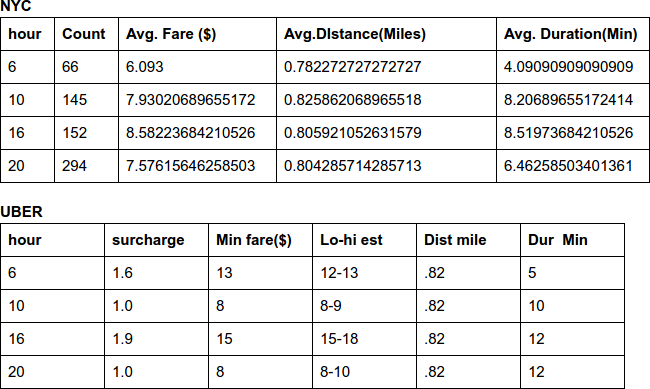
\includegraphics[width=0.7\columnwidth]{figures/one}
\caption{The Image shows the Comparison for the first location with NYC.%
}
\end{center}
\end{figure}

\begin{figure}[h!]
\begin{center}
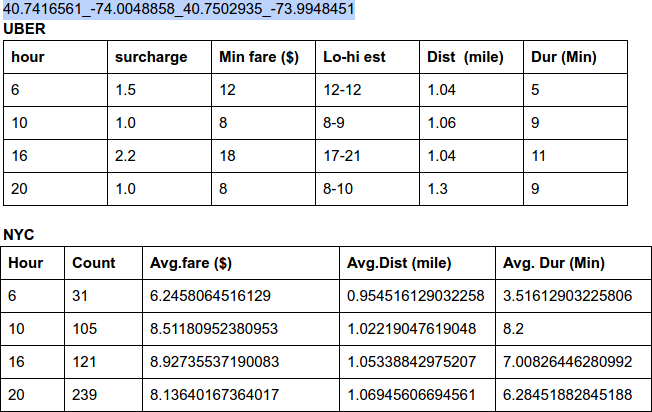
\includegraphics[width=0.7\columnwidth]{figures/two}
\caption{The Image shows the Comparison for the second location with NYC.%
}
\end{center}
\end{figure}

\section{Estimate , High Estimate ,Fare Calculation and Use of Surcharge!}
By making the above tables and doing the analysis we found out that,
\\\textbf{LOW ESTIMATE}
\\ Minimum Fare or Low estimate are equal in almost 100 percent cases.
\\ Low Estimate = (Base Minimum fare) * Surcharge
\\ Like in first case For Uber x, Timezone 6,Low Estimate = 8 * 1.6 = 13
\pagebreak
\\\textbf{HIGH ESTIMATE}
\\ This depends on two factors Duration and Distance
\\ At the time query is made, uber makes the query in the google traffic api and find the two times
\\ Time factor = (Time(with traffic) - Time(without traffic)) * price/dur 
\\ Distance factor = (Distance(More maybe due to traffic) - Distance(Normal)) * price/distance
\\ Total factor  = (Time factor + Distance Factor)*surcharge
\\ Like in second example in Timezone 16, Total factor = (11-6)*0.35*2.2 = 3.85 
\\ Hence , High estimate = Low Estimate + total factor = 17 +3.85 = 21
\\\textbf{FINAL FARE CALCULATION}
\\ Total Fare = (Base Fare + Duration*(price/min) +Distance*(price/mile) )*surcharge
\\ Updated Min fare = Base Min fare * Surcharge
\\if Total Fare < Updated Min Fare then Total Fare = Updated Min Fare
\\ Even if fare is less than minimum , this is charged to the user.
\\ So even if , we use uber for very small rides , uber will charge us the whole amount.
\\ This formula was also verfied over all the data collected for four timezones and it was true in 99.99 percent cases
\\\textbf{SURCHARGE}
\\ This tells us that by using the dynamic surcharge which changes depending on location and time, uber is able to earn most of its revenue.
\\ It increases the Minimum Fare and thus earns the most even in very short trips.
\\ Graph was plotted where only the small trips where the Total Fare was less than Minimum Fare and Uber Earned More
\\ This was plotted for all Timezones 6,10,16,20
The plot is given below:

\begin{figure}[h!]
\begin{center}
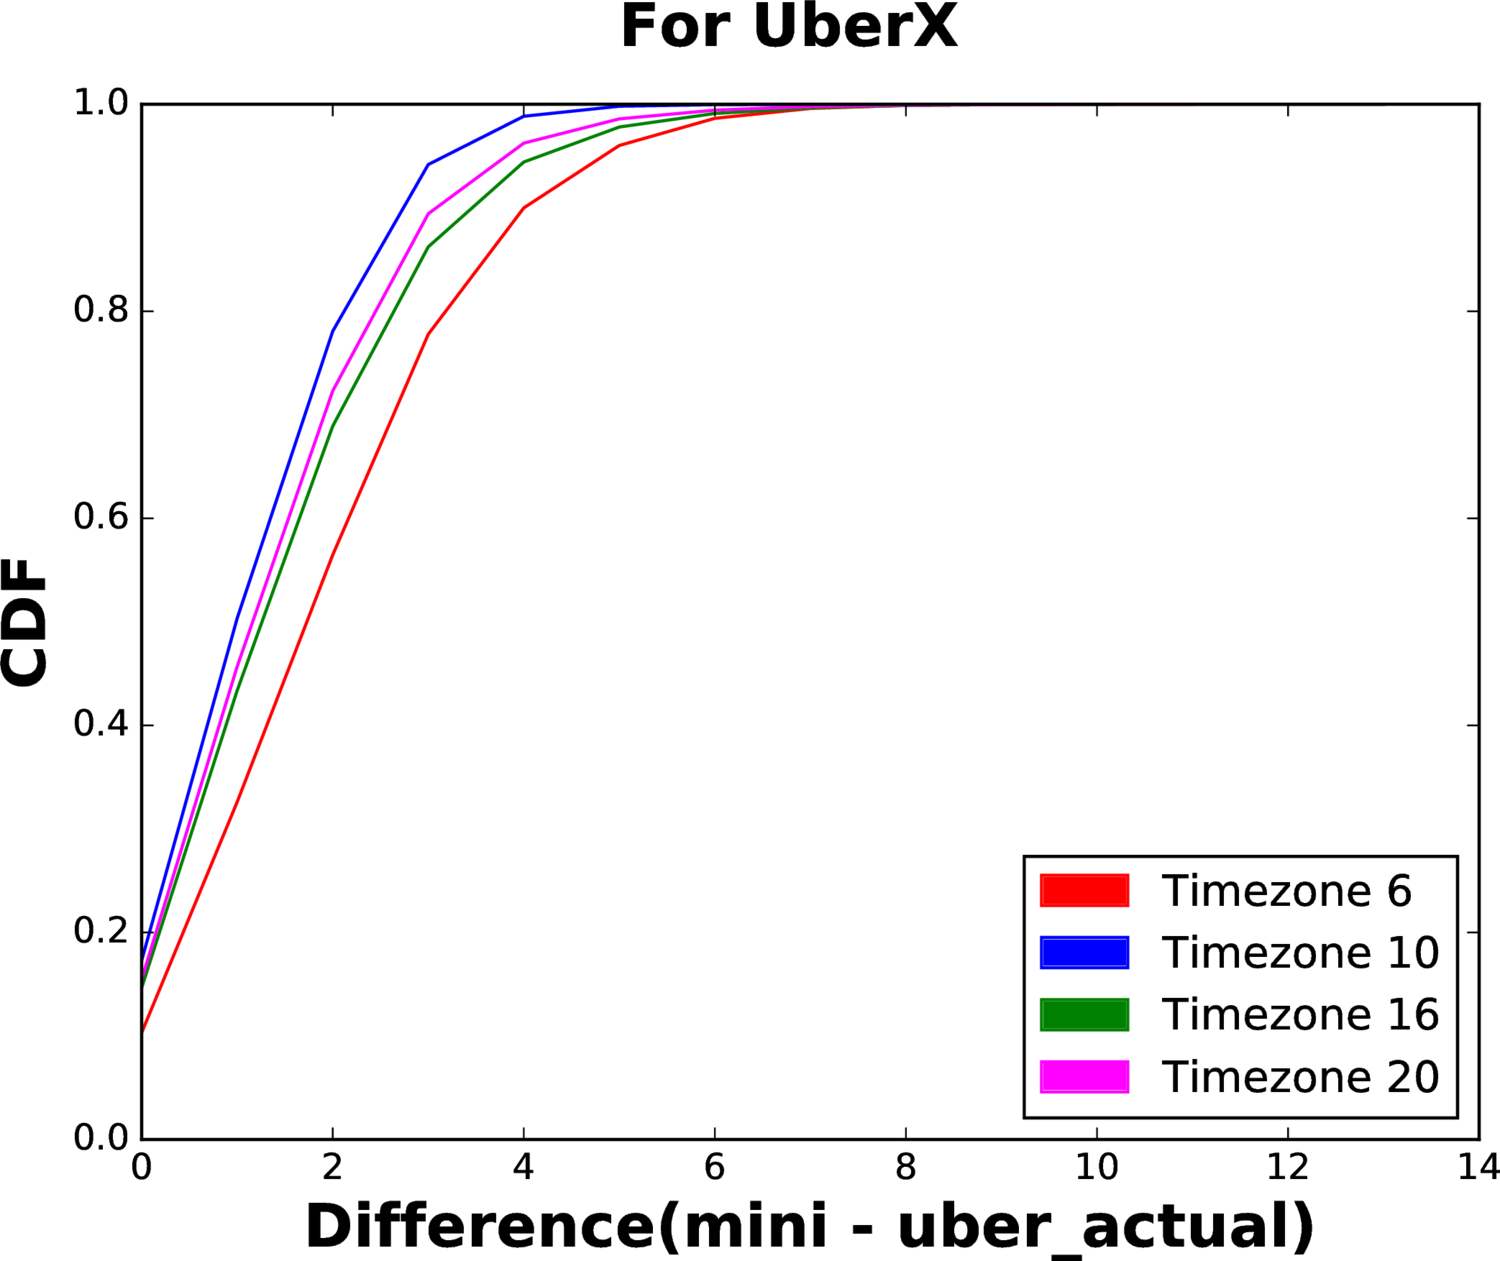
\includegraphics[width=0.7\columnwidth]{figures/three}
\caption{%
}
\end{center}
\end{figure}

\section{Comparison of Uber Fare with NYC fare ! Plotting the Cumulative distribution function(CDF) !}


First the intersection of all the Timezone 6,10,16,20 locations is taken called the \textbf{Candidate Set}
\\Next,we make a json file which stores like key is location and values is difference between the fare
\\ uber\_fare = (high\_estimate +low\_estimate)/2 - nyc\_fare;
\\ DO this for all services:
\\
\linebreak
\linebreak
\linebreak
\noindent
{\it Example Result}
\begin{verbatim}
"40.690346_-73.960293_40.6904473_-73.9787192": {
        "diff\_black": 8.016,
        "diff\_family": 17.516,
        "diff\_pool": 7.516,
        "diff\_suv": 18.016,
        "diff\_x": 7.516,
        "diff\_xl": 11.516 }
\end{verbatim}
\begin{enumerate}
\item Next task is finding the cdf for all the services. 
\item DO this for each service of Uber.
\item round off the differences and convert to int.
\item Find the frequency of each difference. Sum it up.
\item Divide the freq/sumofallfreq in the list.
\item Find the cumulative sum yaxis[i] = yaxis[i] + yaxis[i-1]
\item And now plot the line with 
\item Differnece in Fare (X axis)
\item CDF (Y axis) (Ranging between 0 to 1)
\item Doing this for the four  Timezones Gives us four plots with 6 cdf lines each for each service of uber.
\end{enumerate}
\textbf{The Four plots are given below:}


\begin{figure}
\begin{center}
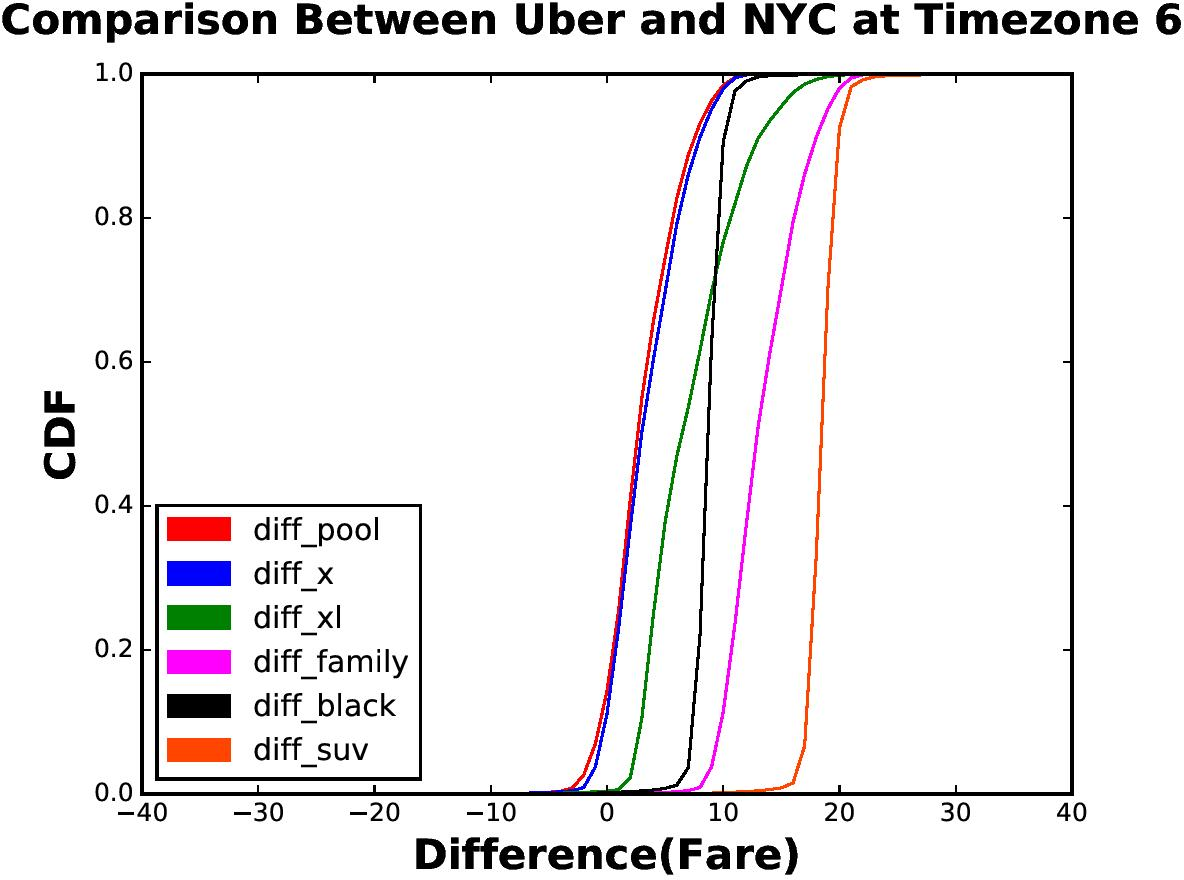
\includegraphics[width=0.7\columnwidth]{figures/four}

\end{center}
\end{figure}

\begin{figure}
\begin{center}
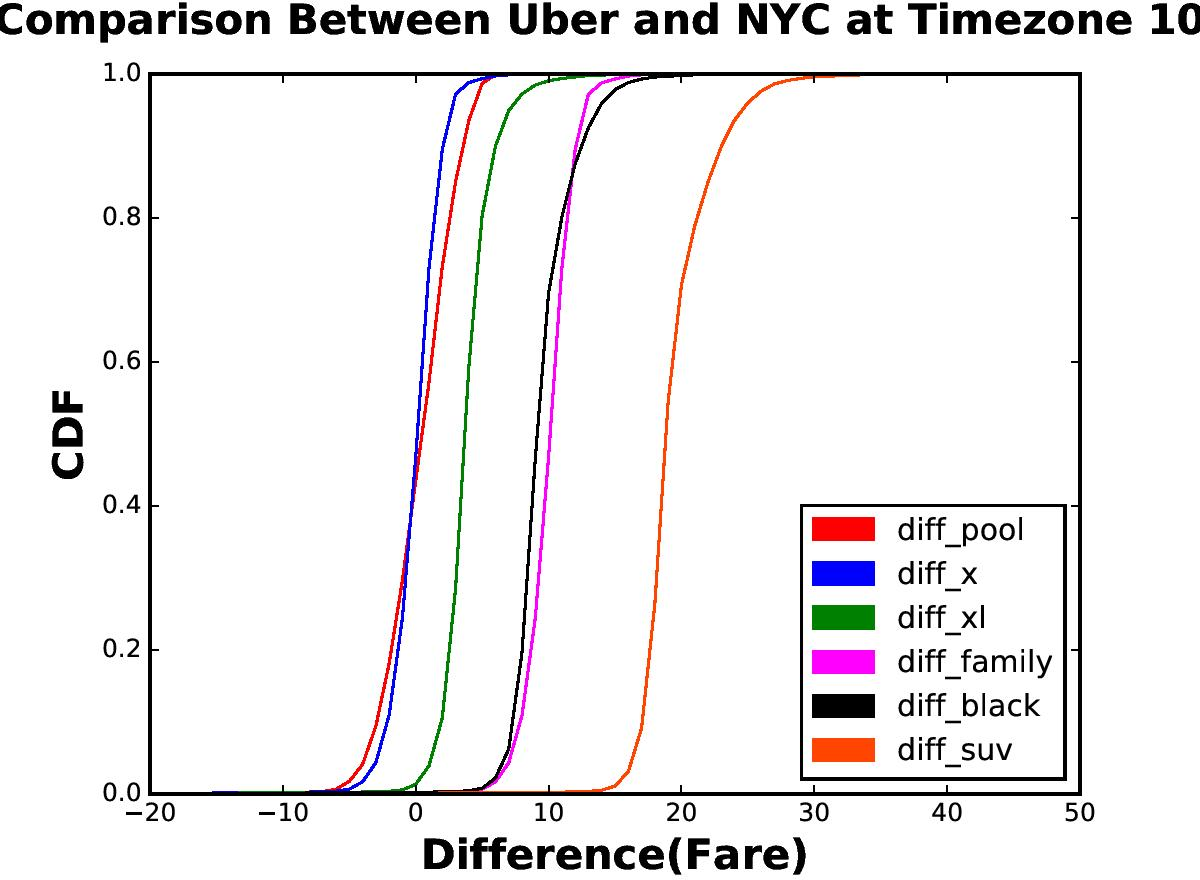
\includegraphics[width=0.7\columnwidth]{figures/five}

\end{center}
\end{figure}

\begin{figure}
\begin{center}
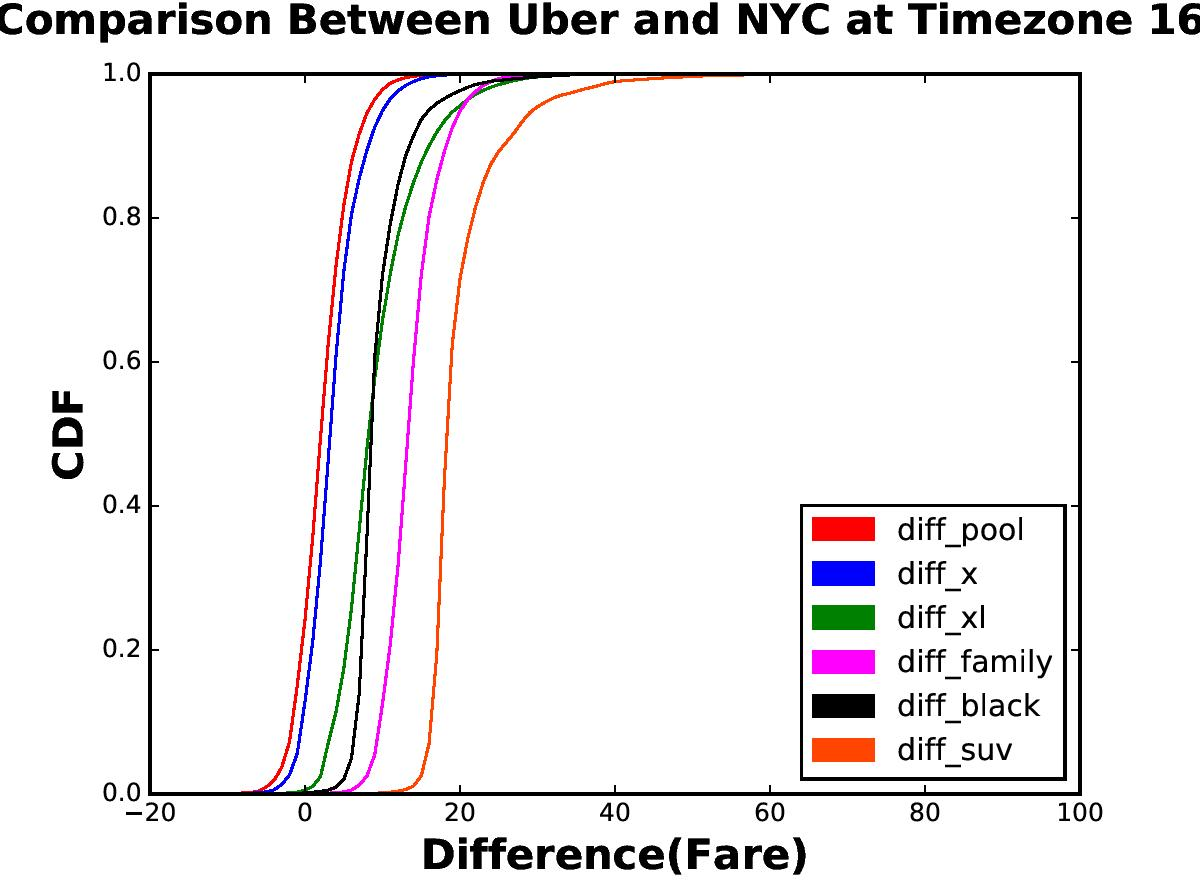
\includegraphics[width=0.7\columnwidth]{figures/six}

\end{center}
\end{figure}

\begin{figure}
\begin{center}
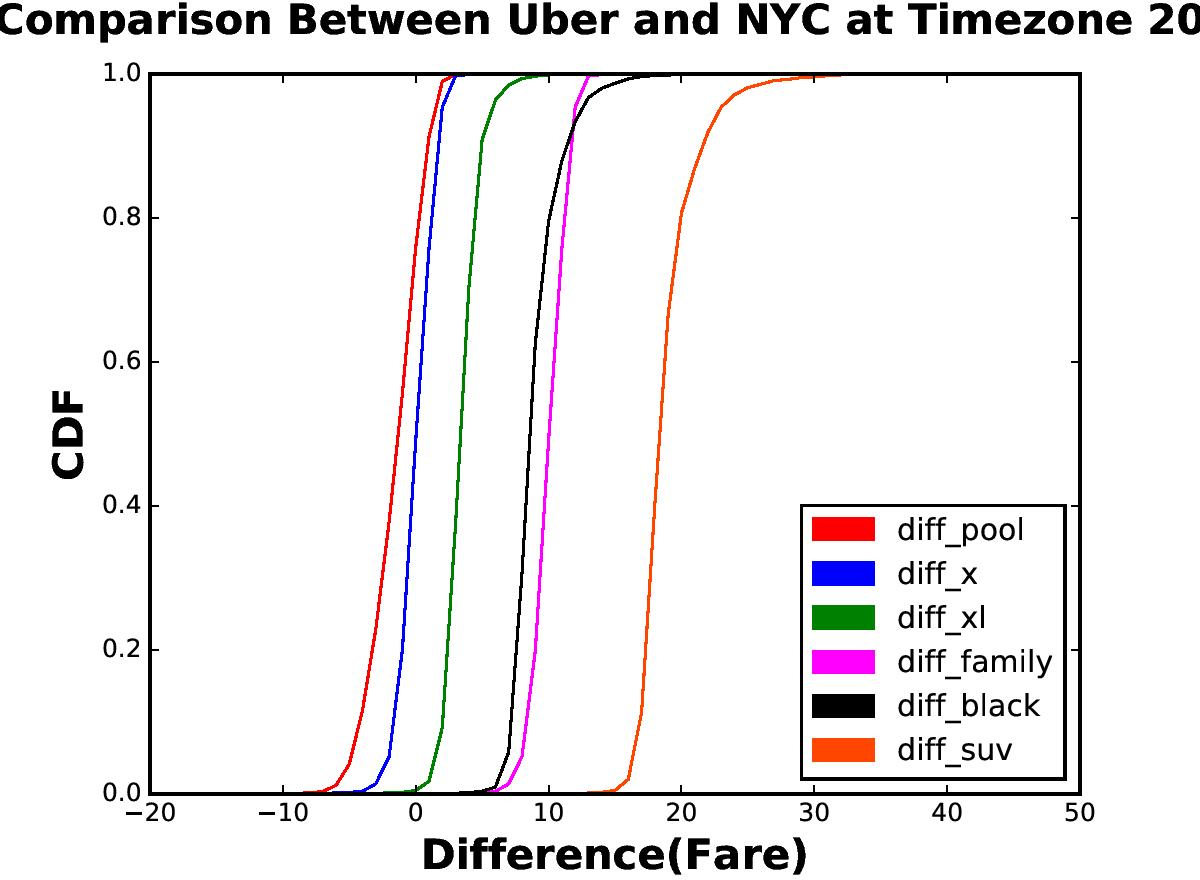
\includegraphics[width=0.7\columnwidth]{figures/seven}

\end{center}
\end{figure}

\pagebreak
\section{Interpretation On looking at the graphs!}

Few interpretation Points: (Basic Analysis is Done)
\\Red line is Uber\_pool that is  cheapest service of uber.
\\At Tiimezone 6, it is mostly costlier than NYC most of the part of line after 0 difference.
\\At Timezone 10 , diff is mostly -ve or 0, meaning Uber is cheaper or almost equal to NYC fare
\\Similar pattern is observed at timezone 16(Uber is costly) and Timezone20(Uber is cheaper or equal)
\\In the early morning , Uber is Costlier and fare decreases during the day. 
\\At timezone 6, It is more costlier than Timezone 16, Then fare decreases as we approach night (Timezone 20).
\\ For Commuters or Daily goers 
\\ People who go early morning and return in the evening daily that is  Commuters, uber will be costlier as uber is charging more in the early morning and in the evening time as compared to NYC.Thus, Uber is earning more as it is charging more at the times of higher demand. Thus , Fare depends upon the customer demand here.
\\Overall, NYC taxi would be cheaper for the commuters.
\\But at other times i would say uber is cheaper or more or less the same fare as compared to NYC.
\\ These are just the first impressions by looking at the graph.


\section{Making Pickup Dropoff Profile!}

Now we used the NYC Dataset
\\First Get all the pickup locations in the dataset
\\ Next Get all the dropoff locations in the dataset
\\ Find their union (22609 locations)
\\ Now we will generate a json file such that
\\ key will be a location and further two keys pickup and dropoff each having value
\\ as a list of 24 values for 0 to 23 timezones
\\ Each value is actually count or popularity of that location.
\\ If not present in pickup or dropoff , put value is equal to null.
\\ Here also keep the popular locations only which have count > 5
\\ Here also large number of locations are there, union list was split and run in parallel.
\textbf{\\Query: Giving input a list of locations and getting result in the form of table in which there are many rows for single location but for different timezones.
\\select pickup,timezone,count(pickup) from nyctaxi where pickup in (location list) group by pickup,timezone;}
{\it \\Example Result of profile}
\begin{verbatim}
  "40.690175_-73.955266": {
        "dropoff": [
            0,
            0,
            1,
            2,
            3,
            1,
            0,
            1,
            0,
            0,
            1,
            0,
            0,
            0,
            0,
            2,
            0,
            0,
            2,
            2,
            1,
            1,
            0,
            3
        ],
        "pickup": [
            37,
            27,
            15,
            9,
            7,
            0,
            0,
            0,
            0,
            0,
            0,
            0,
            6,
            0,
            0,
            6,
            0,
            10,
            14,
            11,
            19,
            20,
            33,
            40
        ]
    }

\end{verbatim}


\section{Population Estimator!}

Using the popularity of all the locations at different timezones.
At present, Suppose timezone is fixed at 16 and use only pickup locations.
We will use the data for all the locations and want to train our model such that if any new location is given as input, the model is able to predict the value of popularity.
\\
When a new location is given,we will draw a circle of radius(r) 0.1 mile and if that contains atleast 1 known location, we will use them to predict our popularity.
If not , then increase the radius by .1 and  again check , maximum  value of radius is 1 mile.
Simple find the average of the all the locations inside the radius and then multiply it by a factor(1.0 minus r).This will be the popularity of the new location.
  
\section{Surcharge Analysis or Prediction!}


\textbf{Statistics How much percentage Surcharge is there ?}
\begin{enumerate}
\item Percentage of surcharge Timezone 6  is 58.1266427718 (36489 out of 62775)
\item Percentage of surcharge Timezone 10 is 6.00644354684 (12491 out of 207960)
\item Percentage of surcharge Timezone 16 is 90.3482314231 (151570 out of 167762)
\item Percentage of surcharge Timezone 20 is 0.218568704613 (431 out of 197192)
\end{enumerate}

\textbf{Observation}

We can see a pattern in the early morning there is surcharge then it decreases during the day,then again it grows very rapily at around 4 pm and at the night it becomes almost zero percent.

\section{Surcharge Experiment!}


By going through the journal paper [1], we found out that they did a surchrage experiment to predict the value of surcharge given a location.They trained their model using Average Surcharge Over a pickup location in a period of 24*7 that is 168  hours and Demand at that location or cell was found out using Different datasets NYC,FourSquare and others.The prediction was done using the DecisionTree Regressor with max depth of three and Leave Out One Validation was used. They got different MSE for each dataset they used for knowing about the demand at that location.They also found out correlation of surcharge with pickup location that was \textbf{0.96} and for dropoff it was \textbf{0.57}. This tells us that surcharge depends more on the pickup location.Assuming uniform effect of dropoff location on surcharge we can predict the value of surcharge at a test location.

\section{Surcharge Estimator!}
  
 Next part is we want to estimate the surcharge , we will train our model using the pickup profile we had calculated.
 We want to do weighted least square fit or regression in which the weight parameter is different for each tuple such that when a new location comes, we find the K NEAREST ones and find the result for them and take the average.This average will be our result.
\\Input will be the popularity of the location and model will predict the surcharge.Just a hypothesis,we can apply PCA by transposing the input matrix and find the eigenvalues.
 These values can be used a weights.
 \\ Training Set will have
 \\ Popularity for input location
 \\ Surcharge - 1.0 (Only Measuring Excess Surcharge)
 \\ This way we will be able to train our model and predict the surcharge at the location.
 
\section{Proposed Model}


Using:
\\ \textbf{This model can be created for each timezone and the value can be approximated.}
\\Popularity estimator(Give location input gives out the popularity)
\\Surcharge estimator(Give input popularith gives out the surcharge)
\\These two can be combined to get the result.

\begin{figure}[h!]
\begin{center}
\includegraphics[width=0.7\columnwidth]{figures/eight}
\end{center}
\end{figure}

\section{Other Approaches!}
\textbf{Market Stablization}

Market demand and supply stabilization:
\\Say in a place 10 people are requesting for Uber cabs. But only 5 uber cabs are there so surcharge will be 2.0x. But there are 10 normal yellow cabs are also there but just nearby blocks. And each yellow cab is an independent system so they don’t get to know that 10 people have requested for cabs. So they wait vacant. 
\\Wheras uber cars are a coordinated system monitored by uber. So they on the first hand get to know the demand. And based upon their supply they estimate the surcharge.
\\But in reality in this case there is no gap in demand and supply. Rather  for 10 people 10 yellow+5 uber cabs are there. So there should not be any surcharge.  But in reality uber is benefiting in this case. 
\\But if somehow we could instruct those 10 yellow cars to go to that place then say 4 people use yellow cabs and only 6 people request uber. Then demand/supply become 6/5 = 1.2
So surcharge reduces and the market gets stabilized. 


\section{Things to do!}

Have to implement the proposed model and validate it.
\\This model can be created for all the timezones.
\\ Market Stablization
\\ More improvements

\pagebreak
\section{References:}
\begin{enumerate}
\item Mining open datasets for transparency in taxi transport in metropolitan environments by Anastasios NoulasEmail author, Vsevolod Salnikov, Renaud Lambiotte and Cecilia Mascolo.

\url{https://epjdatascience.springeropen.com/articles/10.1140/epjds/s13688-015-0060-2}
\end{enumerate}
\end{document}

